\noindent \textred{4.}
\textbf{(3 points)} \textit{Vision Transformers.} In HW1 you trained a dense neural network which can classify images from the FashionMNIST dataset. In this problem, you are tasked to achieve the same objective, but using Vision Transformers. Use a patch size of $4\times 4$, 6 ViT layers, and 4 heads. You can adapt the \href{https://github.com/chinmayhegde/dl-demos/blob/71d043eb60df23028a924b59027f6d241e830fde/extra/visual_transformers.ipynb}{Jupyter notebook} provided on Brightspace to train ViTs. \\

\noindent \myAnswer{
The whole PDF exported from Jupyter notebook is attached at the end. The ViT was trained for 20 epochs with learning rate of $1\times 10^{-3}$. Below is the loss and accuracy curve. After training, both training and testing accuracy achieved $\sim 90\%$.
\begin{figure}[!h]
    \centering
    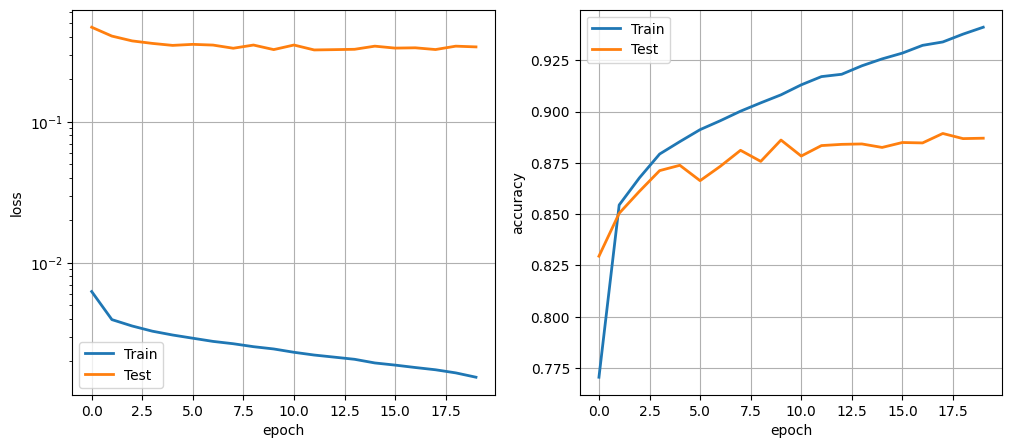
\includegraphics[width=\linewidth]{HWs//HW2//figures/4-1.png}
\end{figure}
\\
Below is the plot of 3 randomly selected samples from the test set with their true labels and predicted results. We can see that most results are correct. Even though the third sample was incorrectly predicted, its prediction still had some components on the true label, \ie, category 0. What's more, the wrongly predict class 6 is ``Shirt", which is close to the true label 0 ``T-Shirt". Therefore, the results are reasonable and interpretable.
\begin{figure}[!h]
    \centering
    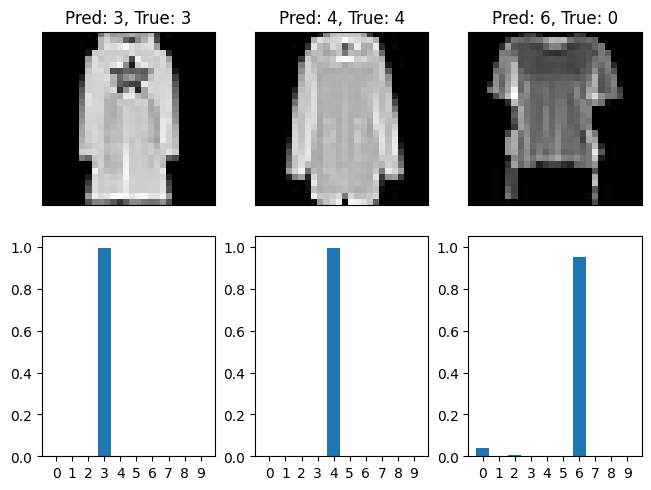
\includegraphics[width=0.7\linewidth]{HWs//HW2//figures/4-2.png}
\end{figure}
}
